\documentclass{standalone}
\usepackage{tikz}

\begin{document}
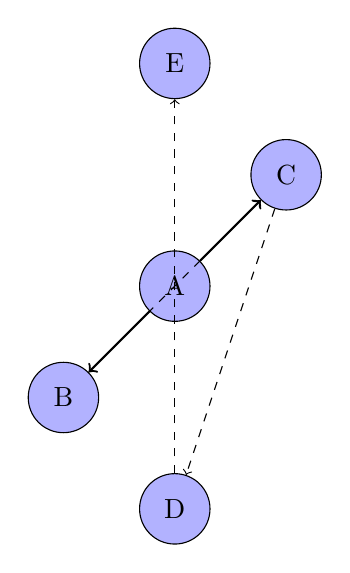
\begin{tikzpicture}[node distance=2cm,
                    every node/.style={circle, draw, fill=blue!30, text width=1.5em, align=center},
                    bold edge/.style={thick,->},
                    dotted edge/.style={dashed,->}]

    % Nodes
    \node (A) {A};
    \node (B) [below left of=A] {B};
    \node (C) [above right of=A] {C};
    \node (D) [below right of=B] {D};
    \node (E) [above left of=C] {E};

    % Edges
    \draw[bold edge] (A) -- (B);
    \draw[bold edge] (A) -- (C);
    \draw[dotted edge] (B) -- (C);
    \draw[dotted edge] (C) -- (D);
    \draw[dotted edge] (D) -- (E);

\end{tikzpicture}
\end{document}